\begin{center}

    \tikzset{every picture/.style={line width=0.75pt}} %set default line width to 0.75pt        
    
    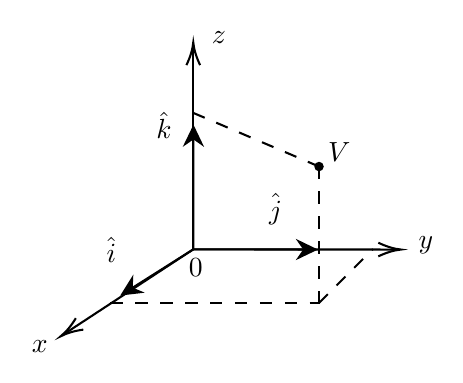
\begin{tikzpicture}[x=0.75pt,y=0.75pt,yscale=-1,xscale=1]
    %uncomment if require: \path (0,214); %set diagram left start at 0, and has height of 214
    
    %Straight Lines [id:da34741946249595057] 
    \draw    (339.92,139.91) -- (340.01,82.83) ;
    \draw [shift={(340.01,79.83)}, rotate = 90.09] [fill={rgb, 255:red, 0; green, 0; blue, 0 }  ][line width=0.08]  [draw opacity=0] (10.72,-5.15) -- (0,0) -- (10.72,5.15) -- (7.12,0) -- cycle    ;
    %Straight Lines [id:da35183475808822884] 
    \draw    (339.92,139.91) -- (397,140) ;
    \draw [shift={(400,140)}, rotate = 180.09] [fill={rgb, 255:red, 0; green, 0; blue, 0 }  ][line width=0.08]  [draw opacity=0] (10.72,-5.15) -- (0,0) -- (10.72,5.15) -- (7.12,0) -- cycle    ;
    %Straight Lines [id:da3444772189505243] 
    \draw    (339.92,139.91) -- (307.26,160.56) ;
    \draw [shift={(304.73,162.16)}, rotate = 327.69] [fill={rgb, 255:red, 0; green, 0; blue, 0 }  ][line width=0.08]  [draw opacity=0] (10.72,-5.15) -- (0,0) -- (10.72,5.15) -- (7.12,0) -- cycle    ;
    %Straight Lines [id:da5975516204182194] 
    \draw    (339.92,139.91) -- (438,140) ;
    \draw [shift={(440,140)}, rotate = 180.05] [color={rgb, 255:red, 0; green, 0; blue, 0 }  ][line width=0.75]    (10.93,-3.29) .. controls (6.95,-1.4) and (3.31,-0.3) .. (0,0) .. controls (3.31,0.3) and (6.95,1.4) .. (10.93,3.29)   ;
    %Straight Lines [id:da30250870787182804] 
    \draw    (339.92,139.91) -- (339.92,42.2) ;
    \draw [shift={(339.92,40.2)}, rotate = 90] [color={rgb, 255:red, 0; green, 0; blue, 0 }  ][line width=0.75]    (10.93,-3.29) .. controls (6.95,-1.4) and (3.31,-0.3) .. (0,0) .. controls (3.31,0.3) and (6.95,1.4) .. (10.93,3.29)   ;
    %Straight Lines [id:da12041369995991924] 
    \draw    (339.92,139.91) -- (277.67,180.72) ;
    \draw [shift={(276,181.82)}, rotate = 326.75] [color={rgb, 255:red, 0; green, 0; blue, 0 }  ][line width=0.75]    (10.93,-3.29) .. controls (6.95,-1.4) and (3.31,-0.3) .. (0,0) .. controls (3.31,0.3) and (6.95,1.4) .. (10.93,3.29)   ;
    %Shape: Circle [id:dp10671391488934368] 
    \draw  [fill={rgb, 255:red, 0; green, 0; blue, 0 }  ,fill opacity=1 ] (398.75,100) .. controls (398.75,99.03) and (399.53,98.25) .. (400.5,98.25) .. controls (401.47,98.25) and (402.25,99.03) .. (402.25,100) .. controls (402.25,100.97) and (401.47,101.75) .. (400.5,101.75) .. controls (399.53,101.75) and (398.75,100.97) .. (398.75,100) -- cycle ;
    %Straight Lines [id:da8040052427893101] 
    \draw  [dash pattern={on 4.5pt off 4.5pt}]  (400.5,100) -- (400.5,170.75) ;
    %Straight Lines [id:da4998664678624216] 
    \draw  [dash pattern={on 4.5pt off 4.5pt}]  (300,165.75) -- (400.5,165.75) ;
    %Straight Lines [id:da42817316260732885] 
    \draw  [dash pattern={on 4.5pt off 4.5pt}]  (400.5,165.75) -- (426.5,139.75) ;
    %Straight Lines [id:da5278231205946351] 
    \draw  [dash pattern={on 4.5pt off 4.5pt}]  (339.92,74.16) -- (400.5,100) ;
    
    % Text Node
    \draw (375,111.6) node [anchor=north west][inner sep=0.75pt]    {$\hat{j}$};
    % Text Node
    \draw (320.64,72.4) node [anchor=north west][inner sep=0.75pt]    {$\hat{k}$};
    % Text Node
    \draw (296.64,132.4) node [anchor=north west][inner sep=0.75pt]    {$\hat{i}$};
    % Text Node
    \draw (336.36,142.8) node [anchor=north west][inner sep=0.75pt]    {$0$};
    % Text Node
    \draw (260.64,182.4) node [anchor=north west][inner sep=0.75pt]    {$x$};
    % Text Node
    \draw (447,132.4) node [anchor=north west][inner sep=0.75pt]    {$y$};
    % Text Node
    \draw (347.44,33.6) node [anchor=north west][inner sep=0.75pt]    {$z$};
    % Text Node
    \draw (403.4,86.8) node [anchor=north west][inner sep=0.75pt]    {$V$};
    
    \end{tikzpicture}

\end{center}